\begin{frame}
\frametitle{Implementing Branch Coverage}

\begin{itemize}
\item Need to count the number of branches executed
\item Could consider each child of an AST, but there are some branches that we don't want to count
\item Could consider all of the blocks of the AST, but there aren't always blocks (case statement, if statement).
\item Need to consider path coverage
\end{itemize}

\end{frame}

\begin{frame}
\frametitle{Implementing Branch Coverage - Creating a CFG}

\begin{figure}
\centering
\begin{minipage}{.3\textwidth}
  \centering
  \lstinputlisting[language=EOL]{code/statements/block.java}
  %\caption{}
  %\label{lst:blockStatement}
\end{minipage}%
\begin{minipage}{.3\textwidth}
  \centering
  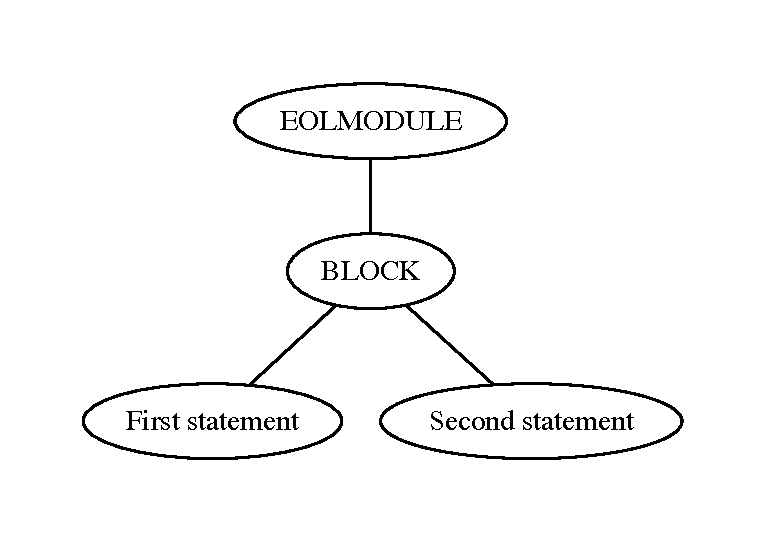
\includegraphics[width=\linewidth]{figures/statements/block_AST.pdf}
   % \caption{}
  %\label{fig:blockAST}
\end{minipage}
\begin{minipage}{.3\textwidth}
  \centering
  \includedot[scale=0.3]{figures/statements/block_CFG}
   % \caption{}
  %\label{fig:blockCFG}
\end{minipage}
\caption{From left to right: The block's code, AST and desired CFG}
\label{fig:block}
\end{figure}

\end{frame}

\begin{frame}
\frametitle{Implementing Branch Coverage - Creating a CFG}

\begin{figure}
\centering
\begin{minipage}{.3\textwidth}
  \centering
  \lstinputlisting[language=EOL]{code/statements/if.java}
  %\caption{}
  %\label{lst:blockStatement}
\end{minipage}%
\begin{minipage}{.3\textwidth}
  \centering
  \includedot[width=\linewidth]{figures/statements/if_AST}
   % \caption{}
  %\label{fig:blockAST}
\end{minipage}
\begin{minipage}{.3\textwidth}
  \centering
  \includedot[scale=0.3]{figures/statements/if_CFG}
   % \caption{}
  %\label{fig:blockCFG}
\end{minipage}
\caption{From left to right: Code for an if statement, its AST and desired CFG}
\label{fig:if}
\end{figure}

\end{frame}

\begin{frame}
\frametitle{Implementing Branch Coverage - Creating a CFG}

\begin{figure}
\centering
\begin{minipage}{.35\textwidth}
  \centering
  \lstinputlisting[breaklines=true,language=EOL]{code/statements/while.java}
  %\caption{}
  %\label{lst:blockStatement}
\end{minipage}%
\begin{minipage}{.3\textwidth}
  \centering
  \includedot[width=\linewidth]{figures/statements/while_AST}
   % \caption{}
  %\label{fig:blockAST}
\end{minipage}
\begin{minipage}{.24\textwidth}
  \centering
  \includedot[scale=0.3]{figures/statements/while_CFG}
   % \caption{}
  %\label{fig:blockCFG}
\end{minipage}
\caption{From left to right: The while loop code (taken from the Epsilon Book), AST and desired CFG}
\label{fig:while}
\end{figure}

\end{frame}

\begin{frame}
\frametitle{Implementing Branch Coverage - Creating a CFG}

\begin{figure}
\centering
\begin{minipage}{.44\textwidth}
  \centering
  \lstinputlisting[breaklines=true,language=EOL]{code/statements/switch2.java}
  %\caption{}
  %\label{lst:blockStatement}
\end{minipage}%
\begin{minipage}{.55\textwidth}
  \centering
  \includedot[scale=0.3]{figures/statements/switch2_CFG}
   % \caption{}
  %\label{fig:blockCFG}
\end{minipage}
\caption{A switch statement and its CFG.}
\label{fig:switch2}
\end{figure}

\end{frame}

\begin{frame}
\frametitle{Implementing Branch Coverage - Conversion Algorithm}

\begin{itemize}
\item Depth First Search
\item Special cases for each statement
\item Interface to add new statements
\end{itemize}
\end{frame}